% Copyright 2026 Sreeram Anil
% SPDX-License-Identifier: CC-BY-4.0
% =============================================================================
%  QUEST — Wahba's problem, Davenport's q-method, attitude (AHRS) family
% =============================================================================
\chapter{Quaternion Estimator for Wahba's Problem (QUEST)}
\label{ch:att-quest}

\section*{At a glance}
\begin{tabular}{@{}l>{\raggedright\arraybackslash}p{0.76\textwidth}@{}}
Family & attitude / AHRS (memory-less baseline) \\
Header & \texttt{include/estkit/attitude/triad\_quest.hpp} \\
Registered name & \texttt{QUEST} \\
State & none: $\bm{q}_k$ is a function of $(\bm{f}_k,\bm{m}_k)$ alone \\
Cost per step & $\approx250$ flops, $\le8$ Newton steps;
  $\SI{214}{\nano\second}$/step, 120\,bytes \\
Primary references & \cite{wahba1965,shusteroh1981,markleymortari2000,keat1977} \\
\end{tabular}

\section{Motivation and aerospace relevance}
TRIAD (Chapter~\ref{ch:att-triad}) resolves the inconsistency between two vector observations by
declaring one of them exact. Wahba~\cite{wahba1965} asked the obvious follow-up question in 1965:
what is the \emph{least-squares} attitude, weighting each observation by its accuracy and using all
of them? Her one-paragraph problem statement generated a forty-year literature; QUEST, the
``QUaternion ESTimator'' of Shuster and Oh~\cite{shusteroh1981}, is the solution that flew --- on
MAGSAT, and on most spacecraft since --- because it replaces an eigen-decomposition with a
scalar Newton iteration and a $3\times3$ matrix polynomial.

Three reasons to include it in an AHRS benchmark. It is the \emph{optimal} single-frame estimator,
so it bounds what any memory-less method can do. Its weights come directly from the sensor noise
model, so it adapts to a change in sensor quality without retuning --- the \texttt{vibration}
scenario below is exactly that experiment. And the matrix $\bm{K}$ it builds is the same object that
appears in the observability analysis of the recursive filters: the conditioning of $\bm{K}$ is why
Chapter~\ref{ch:att-mahony}'s $\bm{M}$ must be positive definite.

\section{Problem statement and assumptions}
Given $m$ pairs of unit vectors $(\bm{b}_i,\bm{r}_i)$ in the BODY and NAV frames with weights
$a_i>0$, $\sum_i a_i=1$, Wahba's problem is
\begin{equation}
\min_{\bm{A}\in SO(3)}\; L(\bm{A}) = \tfrac12\sum_{i=1}^{m} a_i\norm{\bm{b}_i-\bm{A}\bm{r}_i}^2,
\qquad \bm{A}=\bm{R}^\T\ \ (\text{NAV}\to\text{BODY}).
\label{eq:qu-wahba}
\end{equation}
Expanding and using $\norm{\bm{b}_i}=\norm{\bm{r}_i}=1$, $L(\bm{A})=\sum_i a_i - g(\bm{A})$ with the
\emph{gain function}
\begin{equation}
g(\bm{A}) = \sum_i a_i\,\bm{b}_i^\T\bm{A}\bm{r}_i = \sum_i a_i\,\bm{r}_i^\T\bm{R}\bm{b}_i ,
\label{eq:qu-gain}
\end{equation}
so minimising $L$ is maximising $g$. The maximum-likelihood interpretation
(Shuster \& Oh~\cite{shusteroh1981}, Sec.~II): if $\bm{b}_i$ is $\bm{A}\bm{r}_i$ perturbed by an
isotropic tangential error of standard deviation $\sigma_i$ radians, then \eqref{eq:qu-wahba} is the
negative log-likelihood with
\begin{equation}
a_i = \frac{\sigma_{\text{tot}}^2}{\sigma_i^2},\qquad
\sigma_{\text{tot}}^{-2}=\sum_j\sigma_j^{-2},
\label{eq:qu-weights}
\end{equation}
and QUEST is the maximum-likelihood estimator, not merely a least-squares one.

\section{Derivation}

\subsection{Davenport's \texorpdfstring{$\bm{K}$}{K} matrix}
Write the Hamilton quaternion $\bm{q}=[w,\bm{v}]$ (scalar first) for the BODY$\to$NAV rotation, so
\begin{equation}
\bm{R}(\bm{q}) = \big(w^2-\norm{\bm{v}}^2\big)\bm{I} + 2\bm{v}\bm{v}^\T + 2w[\bm{v}]_\times .
\label{eq:qu-Rq}
\end{equation}
Substituting \eqref{eq:qu-Rq} into \eqref{eq:qu-gain} and using
$\bm{r}^\T[\bm{v}]_\times\bm{b}=\bm{v}^\T(\bm{b}\times\bm{r})$ term by term,
\begin{equation}
g(\bm{q}) = \sum_i a_i\Big[(w^2-\norm{\bm{v}}^2)(\bm{r}_i\!\cdot\!\bm{b}_i)
 + 2(\bm{r}_i\!\cdot\!\bm{v})(\bm{v}\!\cdot\!\bm{b}_i)
 + 2w\,\bm{v}^\T(\bm{b}_i\times\bm{r}_i)\Big]
 = \bm{q}^\T\bm{K}\bm{q} ,
\label{eq:qu-quad}
\end{equation}
with, collecting the three groups of terms,
\begin{equation}
\bm{B}=\sum_i a_i\,\bm{b}_i\bm{r}_i^\T,\quad
\sigma=\tr\bm{B},\quad
\bm{S}=\bm{B}+\bm{B}^\T,\quad
\bm{Z}=\sum_i a_i\,(\bm{b}_i\times\bm{r}_i),\quad
\bm{K}=\begin{bmatrix}\sigma & \bm{Z}^\T\\ \bm{Z} & \bm{S}-\sigma\bm{I}\end{bmatrix}\in\real^{4\times4}.
\label{eq:qu-K}
\end{equation}
(The three checks: the $w^2$ coefficient is $\tr(\sum a_i\bm{b}_i\bm{r}_i^\T)=\sigma$; the $2w\bm{v}$
coefficient is $\bm{Z}$; and $2\bm{v}^\T\bm{B}^\T\bm{v}=\bm{v}^\T\bm{S}\bm{v}$ by symmetry.)
Equation~\eqref{eq:qu-K} is written directly for the BODY$\to$NAV Hamilton quaternion used
throughout this family, so no transposition or convention change is needed afterwards --- a
frequent source of sign errors when transcribing Shuster's vector-first, NAV$\to$BODY formulation.

$\bm{K}$ is real symmetric, so it has four real eigenvalues, and
$\max_{\norm{\bm{q}}=1}\bm{q}^\T\bm{K}\bm{q}=\lambda_{\max}$ attained at the corresponding
eigenvector. This is Davenport's $q$-method~\cite{keat1977}: \emph{the optimal quaternion is the
eigenvector of $\bm{K}$ for its largest eigenvalue}. It is exact, it never has a singularity, and it
generalises to any number of observations; the singular-value formulation of
Markley~\cite{markley1988} is the numerically most robust way to evaluate it when $m$ is large.

\subsection{QUEST: \texorpdfstring{$\lambda_{\max}$}{lambda-max} without an eigensolver}
Since $L=\sum_i a_i-\lambda_{\max}$ and the loss is small when the observations are consistent,
$\lambda_{\max}$ is close to $\sum_i a_i = 1$. Shuster and Oh therefore compute it as a root of the
characteristic polynomial, starting from $\lambda_0=\sum_i a_i$. Expanding
$\det(\bm{K}-\lambda\bm{I})$ for the structured $\bm{K}$ of \eqref{eq:qu-K} gives
(\cite{shusteroh1981}, Eq.~(63))
\begin{equation}
\lambda^4-(\alpha_a+\alpha_b)\lambda^2-\alpha_c\lambda+(\alpha_a\alpha_b+\alpha_c\sigma-\alpha_d)=0,
\label{eq:qu-char}
\end{equation}
with
\begin{align}
\kappa&=\tr(\operatorname{adj}\bm{S})=\tfrac12\big((\tr\bm{S})^2-\tr(\bm{S}^2)\big),
&\Delta&=\det\bm{S},\nonumber\\
\alpha_a&=\sigma^2-\kappa, &\alpha_b&=\sigma^2+\bm{Z}^\T\bm{Z},\label{eq:qu-abcd}\\
\alpha_c&=\Delta+\bm{Z}^\T\bm{S}\bm{Z}, &\alpha_d&=\bm{Z}^\T\bm{S}^2\bm{Z}.\nonumber
\end{align}
Newton's method on \eqref{eq:qu-char} converges quadratically from $\lambda_0$; for two
well-conditioned observations one or two iterations suffice.

\subsection{The eigenvector in closed form}
The lower block row of $\bm{K}\bm{q}=\lambda\bm{q}$ with $\bm{q}=[w,\bm{v}]$ reads
$\bm{Z}w=\big((\lambda+\sigma)\bm{I}-\bm{S}\big)\bm{v}$, i.e. with
$\bm{Y}=(\lambda+\sigma)\bm{I}-\bm{S}$,
\begin{equation}
\bm{v}=\bm{Y}\inv\bm{Z}\,w = \frac{\operatorname{adj}(\bm{Y})\bm{Z}}{\det\bm{Y}}\,w .
\label{eq:qu-eig}
\end{equation}
Choosing the (unnormalised) scale $w=\det\bm{Y}$ removes the division entirely. Expanding both
factors with the Cayley--Hamilton identity
$\operatorname{adj}\bm{Y}=\bm{Y}^2-\tr(\bm{Y})\bm{Y}+\tfrac12((\tr\bm{Y})^2-\tr\bm{Y}^2)\bm{I}$ and
$\tr\bm{S}=2\sigma$ gives, after cancellation,
\begin{align}
\alpha&=\lambda^2-\sigma^2+\kappa, &\beta&=\lambda-\sigma, \nonumber\\
\operatorname{adj}\bm{Y}&=\bm{S}^2+\beta\bm{S}+\alpha\bm{I}, &
\det\bm{Y}&=(\lambda+\sigma)\alpha-\Delta =: \gamma,
\label{eq:qu-adj}
\end{align}
so that the optimal quaternion is, in scalar-first BODY$\to$NAV form,
\begin{equation}
\bm{X}=\big(\alpha\bm{I}+\beta\bm{S}+\bm{S}^2\big)\bm{Z},
\qquad
\bm{q}_{\text{opt}} = \frac{1}{\sqrt{\gamma^2+\norm{\bm{X}}^2}}\begin{bmatrix}\gamma\\ \bm{X}\end{bmatrix}.
\label{eq:qu-q}
\end{equation}
This is Shuster and Oh's Eqs.~(66)--(72). Note that \eqref{eq:qu-q} never forms the Gibbs vector
$\bm{X}/\gamma$, which is the singular object in the original derivation: $\gamma=0$ corresponds to
a $180^\circ$ rotation and occurs twice in this mission's yaw profile, but it is harmless here,
because $\bm{X}$ is computed independently of $\gamma$ and the pair $[\gamma,\bm{X}]$ is simply
normalised. The classical ``method of sequential rotations'' is therefore unnecessary in this form.

\paragraph{Degenerate fall-back.}\label{sec:qu-fallback} The formula does fail if $\gamma$ and $\bm{X}$ vanish
\emph{together}, i.e. if $\operatorname{adj}(\bm{Y})\bm{Z}=\bm{0}$ and $\det\bm{Y}=0$. The
implementation detects this by testing $\norm{[\gamma,\bm{X}]}$ and falls back to two steps of
inverse iteration on $\bm{K}-(\lambda+\epsilon)\bm{I}$ (a $4\times4$ LU solve from
\code{linalg.hpp}), seeded with the previous estimate. It has never triggered on this benchmark, but
it costs nothing when it does not.

\subsection{TRIAD as a limit}
With $m=2$ and $a_1\to1$, $a_2\to0$, the maximiser of \eqref{eq:qu-gain} must satisfy
$\bm{R}\bm{b}_1=\bm{r}_1$ exactly and then maximise the residual term --- which is the TRIAD
construction. Shuster and Oh~\cite[Sec.~IV]{shusteroh1981} make this precise: for two observations,
TRIAD is QUEST with an infinite weight ratio, so the two differ only through
\eqref{eq:qu-weights}.

\section{Algorithm}
\begin{algorithm}[H]
\caption{QUEST --- one sampling period (the gyroscope is ignored)}
\begin{algorithmic}[1]
\Require $\bm{f},\bm{m}$; references $\bm{r}_1,\bm{r}_2$; weights $a_1,a_2$ from \eqref{eq:qu-weights}
\State $\bm{b}_1\gets\bm{f}/\norm{\bm{f}}$;\; $\bm{b}_2\gets\bm{m}/\norm{\bm{m}}$
\State $\bm{B}\gets a_1\bm{b}_1\bm{r}_1^\T+a_2\bm{b}_2\bm{r}_2^\T$;\; $\sigma\gets\tr\bm{B}$;\;
       $\bm{S}\gets\bm{B}+\bm{B}^\T$;\; $\bm{Z}\gets a_1\bm{b}_1\times\bm{r}_1+a_2\bm{b}_2\times\bm{r}_2$
\State $\kappa\gets\tfrac12((\tr\bm{S})^2-\tr\bm{S}^2)$;\; $\Delta\gets\det\bm{S}$;\;
       $(\alpha_a,\alpha_b,\alpha_c,\alpha_d)\gets$ \eqref{eq:qu-abcd}
\State $\lambda\gets a_1+a_2$
\For{$j=1,\dots,J$} \Comment{Newton on \eqref{eq:qu-char}, $J=8$}
  \State $\lambda\gets\lambda-\dfrac{\lambda^4-(\alpha_a+\alpha_b)\lambda^2-\alpha_c\lambda+(\alpha_a\alpha_b+\alpha_c\sigma-\alpha_d)}{4\lambda^3-2(\alpha_a+\alpha_b)\lambda-\alpha_c}$;\;
        \textbf{break if} converged
\EndFor
\State $\alpha\gets\lambda^2-\sigma^2+\kappa$;\; $\beta\gets\lambda-\sigma$;\;
       $\gamma\gets(\lambda+\sigma)\alpha-\Delta$;\;
       $\bm{X}\gets(\alpha\bm{I}+\beta\bm{S}+\bm{S}^2)\bm{Z}$
\State \textbf{if} $\norm{[\gamma,\bm{X}]}$ negligible \textbf{then} inverse iteration on $\bm{K}$
\State $\bm{q}_k\gets[\gamma,\bm{X}]/\norm{[\gamma,\bm{X}]}$
\Ensure $\bm{q}_k$
\end{algorithmic}
\end{algorithm}

\section{Application to the benchmark flight}
The weights are derived from the configured sensor noise through \eqref{eq:qu-weights}: the
direction error of a vector measurement of magnitude $\norm{\bm{v}}$ with per-axis noise $\sigma$ is
$\sigma/\norm{\bm{v}}$ radians, so $\sigma_1=\sigma_a/g$ and $\sigma_2=\sigma_m/B$. On the nominal
scenario this gives
\begin{equation}
\sigma_1=\frac{0.05}{9.807}=\SI{5.1e-3}{\radian},\quad
\sigma_2=\frac{0.5}{48}=\SI{10.4e-3}{\radian}
\;\Longrightarrow\;
a_1=0.807,\ a_2=0.193 ,
\label{eq:qu-wnom}
\end{equation}
and on \texttt{vibration}, where the harness raises the configured accelerometer noise to
$\SI{1.05}{\metre\per\second\squared}$, $\sigma_1=\SI{107e-3}{\radian}$ and the weights become
$a_1=0.009$, $a_2=0.991$: the estimator hands the problem to the magnetometer \emph{without being
retuned}. No other estimator in this family adapts to the configuration this directly, and the
benchmark measures the consequence below.

Eight Newton iterations are allowed with a relative break at $10^{-12}$; in practice one or two are
executed.

\section{Implementation notes}
Per step: two outer products and two cross products ($\approx24$ MACs), $\bm{S}^2$ (27),
$\det\bm{S}$ (9 explicit, not via LU), three quadratic forms in $\bm{Z}$ ($\approx30$), the Newton
loop ($\approx10$ flops per iteration) and the $3\times3$ polynomial in \eqref{eq:qu-q} ($\approx30$):
about 250 flops with a single \code{sqrt} beyond the measurement normalisations. Measured
$\SI{214}{\nano\second}$/step, about $66\,\%$ more than TRIAD and still under a quarter of a
microsecond; \code{sizeof} is 120\,bytes, identical to TRIAD because the two share a class and
neither stores anything beyond the last quaternion and the weights.

Numerical hygiene: $\det\bm{S}$ is expanded in closed form rather than by LU, so there is no
pivoting and no failure branch; the Newton loop breaks if $\abs{f'}<10^{-12}$ and is bounded by
$J=8$; \eqref{eq:qu-q} is guarded by a finiteness and magnitude test with the inverse-iteration
fall-back described above; the step is skipped entirely if either measurement magnitude is below
$10^{-6}$. No NaN or infinity was produced on any of the six scenarios
($1.6\times10^{6}$ samples over three seeds). The single-precision build reproduces the
double-precision mission RMS to four digits.

The limitation is structural and shared with TRIAD: no state, no gyroscope, no memory. QUEST is the
best possible \emph{instantaneous} answer, which on a manoeuvring aircraft is not a good answer.

\section{Benchmark results}
% Copyright 2026 Sreeram Anil
% SPDX-License-Identifier: CC-BY-4.0
\begin{table}[H]\centering\footnotesize\setlength{\tabcolsep}{3.5pt}\caption{QUEST: attitude benchmark (mean over seeds; all angles in degrees; $t_\mathrm{conv}$: first time the attitude error stays below 2$^\circ$ for 30\,s; bias RMSE in deg/s; 120 bytes of state).}\label{tab:imu_QUEST}
\begin{tabular}{lrrrrrrrrcr}\toprule scenario & RMS & roll & pitch & yaw & max & RMS$_\mathrm{ss}$ & $t_\mathrm{conv}$ [s] & bias RMSE & lost & ns/step \\ \midrule
nominal & 19.22 & 8.68 & 1.44 & 17.18 & 87.7 & 21.18 & -- & 1.03 & yes & 214 \\
init\_error & 19.22 & 8.68 & 1.44 & 17.18 & 87.7 & 21.18 & -- & 1.03 & yes & 213 \\
gyro\_bias & 19.22 & 8.68 & 1.44 & 17.18 & 87.7 & 21.18 & -- & 3.80 & yes & 215 \\
mag\_disturbance & 20.63 & 8.69 & 1.44 & 18.73 & 87.7 & 21.18 & -- & 1.03 & yes & 215 \\
vibration & 25.89 & 9.10 & 4.93 & 24.28 & 179.7 & 27.94 & -- & 1.03 & yes & 225 \\
high\_dynamics & 20.63 & 9.12 & 1.54 & 18.57 & 138.8 & 22.60 & -- & 1.03 & yes & 216 \\
\bottomrule\end{tabular}\end{table}

\begin{figure}[H]\centering
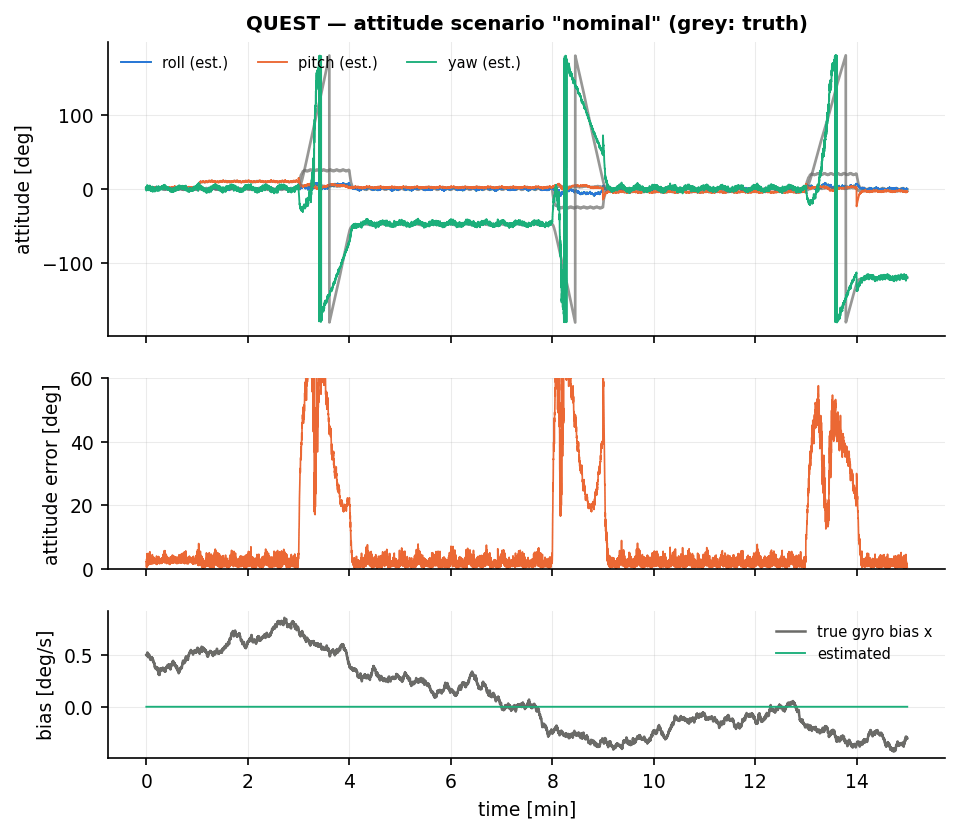
\includegraphics[width=\textwidth]{figures/imu_QUEST_nominal.png}
\caption{QUEST on the nominal mission: the optimal single-frame solution, which during the
coordinated turns is optimally wrong.}
\end{figure}
\begin{figure}[H]\centering
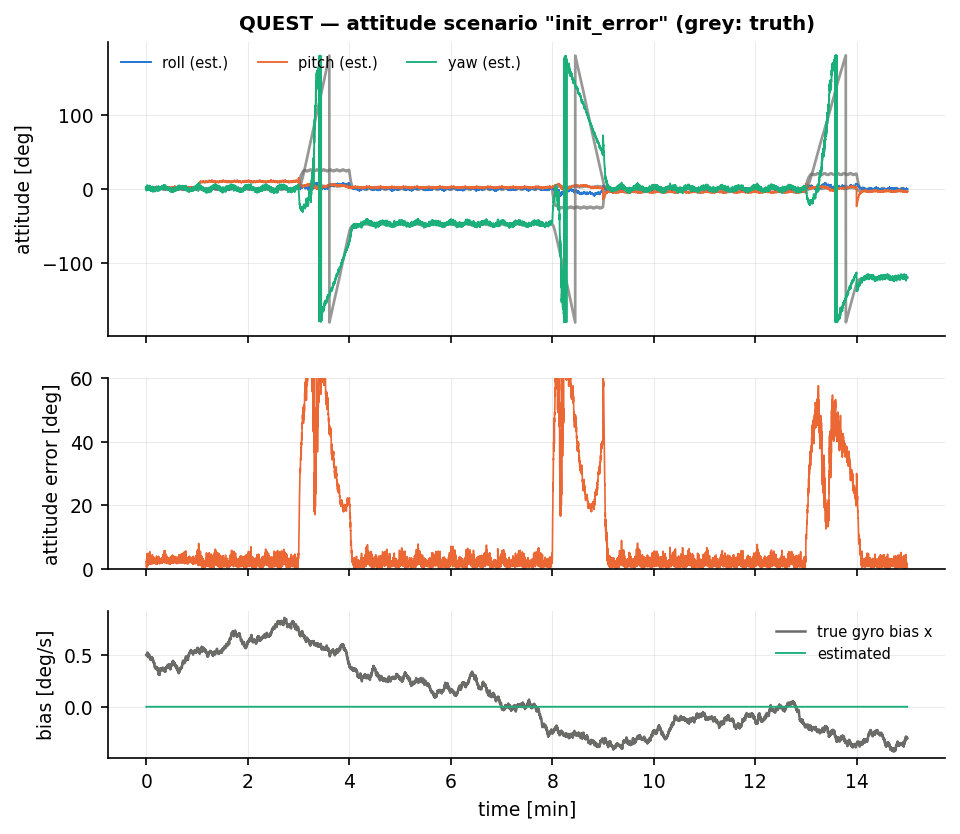
\includegraphics[width=\textwidth]{figures/imu_QUEST_init_error.png}
\caption{QUEST with a $46.6^\circ$ initial error, which it ignores: the trace is identical to the
nominal one.}
\end{figure}

On \texttt{nominal} QUEST gives $\text{RMS}=\SI{19.22}{\degree}$ (roll $8.68$, pitch $1.44$, yaw
$\SI{17.18}{\degree}$), $\text{RMS}_{\text{ss}}=\SI{21.18}{\degree}$, peak $\SI{87.7}{\degree}$ and
$\SI{214}{\nano\second}$/step at 120\,bytes. Like TRIAD it returns \emph{identical} numbers on
\texttt{init\_error} and on \texttt{gyro\_bias}, since it uses neither the initial condition nor
the gyroscope, and its bias RMSE column simply reports the true bias magnitude ($1.03$ and
$\SI{3.80}{\degree\per\second}$). Per phase (seed~1),
\[
2.76\;/\;2.58\;/\;\mathbf{44.42}\;/\;2.52\;/\;\mathbf{42.32}\;/\;2.50\;/\;\mathbf{35.86}\;/\;2.04
\ \SI{}{\degree}
\]
for take-off / climb / turn\,1 / cruise / turn\,2 / descent / turn\,3 / final. The interpretation is
the one given in Chapter~\ref{ch:att-triad} and needs no repetition: in unaccelerated flight the
instantaneous solution is a $\SI{2.5}{\degree}$ device --- close to what the sensors themselves
permit --- while during the three coordinated turns the accelerometer reports zero bank and the
$65^\circ$ magnetic dip amplifies the resulting tilt error into the heading by $\tan I=2.14$.

Table numbers are three-seed means; the variants below are single-seed (seed~1) diagnostics.

\paragraph{QUEST versus TRIAD.} Optimal weighting buys $\SI{0.37}{\degree}$ on \texttt{nominal}
($19.22$ against $\SI{19.59}{\degree}$) and redistributes the error sensibly (roll $8.68$ against
$9.37$). That is a small return, and the reason is \eqref{eq:qu-wnom}: at $a_1=0.807$ the optimal
solution is already close to the accelerometer-primary TRIAD limit, so the two nearly coincide. It
buys more where the weights are far from that limit: on \texttt{vibration} QUEST gives
$\SI{25.89}{\degree}$ against TRIAD's $\SI{27.26}{\degree}$, its pitch RMS is $4.93$ against $6.23$,
and its outlier count is $964$ samples above $90^\circ$ against TRIAD's $986$. This is the
\emph{adaptivity} experiment: the configured accelerometer noise rises by a factor of 21, the
weights swing from $(0.81,0.19)$ to $(0.01,0.99)$ automatically, and the estimator degrades by
$\SI{6.7}{\degree}$ instead of $\SI{7.7}{\degree}$. Forcing equal weights $a_1=a_2=0.5$ gives
$\SI{18.79}{\degree}$ on nominal but $\SI{26.18}{\degree}$ on vibration --- better on the scenario it
happens to suit, worse where the weighting matters, which is the usual fate of a fixed tuning.

\paragraph{The Newton iteration earns its place.} Truncating the iteration degrades the result
measurably: $J=8$ (registered) gives $\SI{19.23}{\degree}$, $J=1$ gives $\SI{20.05}{\degree}$, and
$J=0$ --- i.e. the common approximation $\lambda_{\max}\approx\sum_i a_i$, exact only for consistent
observations --- gives $\SI{24.32}{\degree}$ with a peak of $179.9^\circ$. On this mission the
observations are grossly inconsistent for a fifth of the flight, so $\sum_i a_i$ is a poor estimate
of $\lambda_{\max}$ and the closed form \eqref{eq:qu-q} evaluated at the wrong $\lambda$ is not even
a rotation-optimal answer. Two iterations recover essentially all of it, and the degenerate
fall-back of \S\ref{sec:qu-fallback} never triggered.

\paragraph{The collinearity degeneracy.} Like TRIAD, QUEST produces large outliers on
\texttt{vibration}: $964$ of $9\times10^4$ samples ($1.1\,\%$) exceed $90^\circ$, and the peak is
$179.8^\circ$. The cause is the conditioning of $\bm{K}$, not of the algorithm: at
$t=\SI{488.17}{\second}$, in a $-24.75^\circ$ banked turn, the measured directions are $176.1^\circ$
apart while the references are $155^\circ$ apart, so $\bm{S}-\sigma\bm{I}$ is nearly rank-deficient
in the plane containing both and the maximiser of \eqref{eq:qu-quad} is nearly degenerate. No
weighting can repair an observation geometry in which the two measured directions are almost
anti-parallel; only a gyroscope can, which is the entire argument for the filters in the rest of
this family.

\paragraph{Other scenarios.} \texttt{mag\_disturbance} costs $\SI{1.4}{\degree}$ ($20.63$), entirely
in yaw ($17.18\to\SI{18.73}{\degree}$) as expected for a horizontal field offset;
\texttt{high\_dynamics} costs $\SI{1.4}{\degree}$ ($20.63$, peak $138.8^\circ$). Both scenarios set
the \texttt{lost} flag and neither converges under the harness's $2^\circ$-for-$\SI{30}{\second}$
criterion --- correct descriptions of a memory-less estimator on this mission, not numerical
failures.

\section{Summary}
QUEST is the optimal single-frame attitude estimator: maximum likelihood under isotropic tangential
noise, closed form, $\SI{0.21}{\micro\second}$/step, 120\,bytes, and weights that follow the sensor
noise model with no tuning. Use it for coarse alignment, for initialising a recursive filter, for
star-tracker-style problems where the observations really are simultaneous and independent, and as
the honest optimum against which any memory-less claim must be measured. On this mission it beats
TRIAD by $\SI{0.37}{\degree}$ in nominal conditions and by $\SI{1.4}{\degree}$ under vibration ---
the payoff of weighting is largest exactly when the sensors differ most --- but both remain
$\SI{17}{\degree}$ behind the six-state filters and $\SI{17}{\degree}$ behind a
$\SI{132}{\nano\second}$ gated Mahony observer, because the missing ingredient is not a better
algebraic solution, it is the time axis.
